\chapter{Diagramme de classes participantes}

\section{Introduction}

\begin{figure}[ht]
	\centering 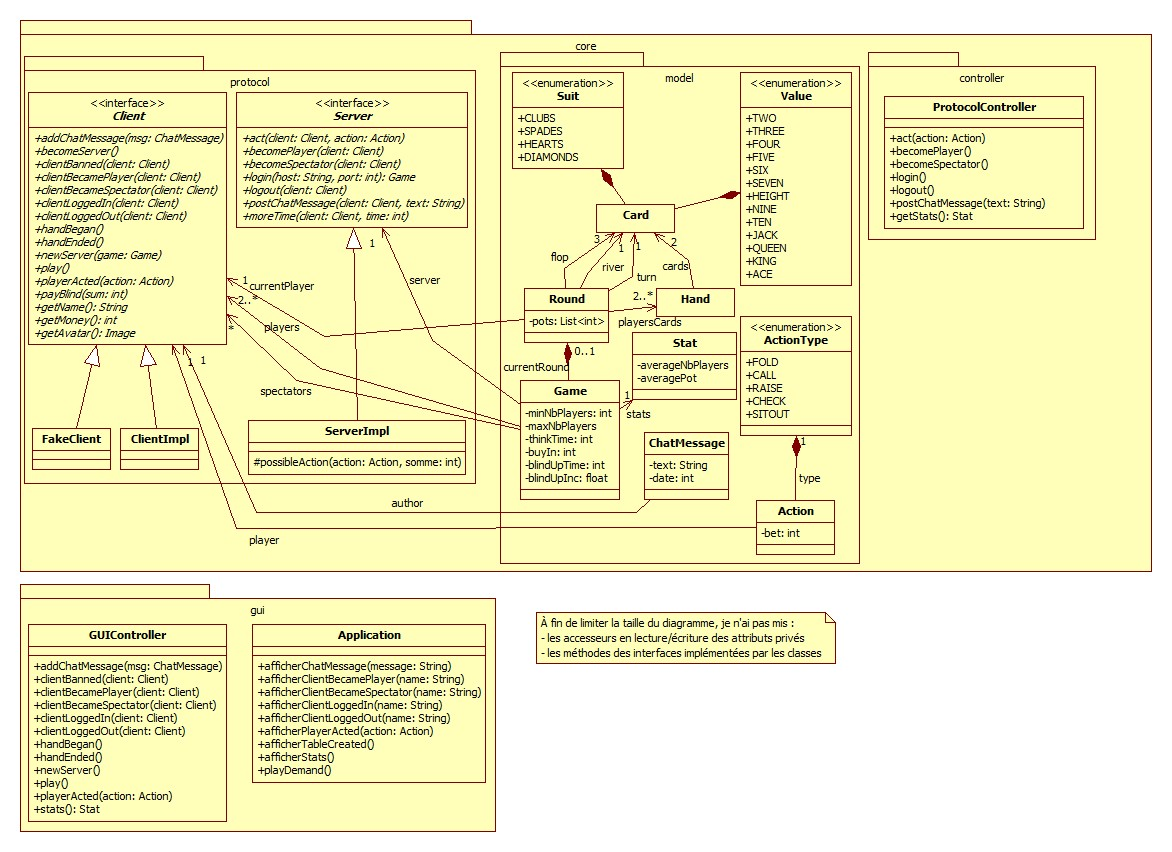
\includegraphics[width=1.50\linewidth, angle=90]{figures/ClassDiagram.jpg}
\end{figure}
\clearpage

L'application est divisée en deux parties :
\begin{itemize}
	\item un package \texttt{core} gérant la communication avec les autres applications
	\item un package \texttt{gui} gérant l'interface graphique et la communication avec l'utilisateur
\end{itemize}

Elle suit une architecture MVC :
\begin{itemize}
	\item la vue est dans le package \texttt{gui}
	\item le modèle est dans le package \texttt{core.model}
	\item les contrôleurs sont répartis dans \texttt{core.controller} et \texttt{gui}.
	En effet, il y a deux catégories d'actions à réaliser : lorsque l'utilisateur fait quelque chose (auquel cas \texttt{ProtocolController} est utilisé pour envoyer l'information au serveur) et lorsque que le serveur demande quelque chose à l'application (auquel cas \texttt{GUIController} est utilisé).
	À ceci est rajouté \texttt{core.protocol} qui se charge de l'implémentation du protocole.
\end{itemize}

\section{Détail des packages}

\subsection{core.protocol}

Il regroupe les objets utilisé par RMI pour communiquer.

Les interfaces \texttt{Client} et \texttt{Server} regroupent toutes les méthodes appelables respectivement par le serveur et par les clients.

Afin de gérer les déconnexions des joueurs, \texttt{Client} dispose de deux implémentations : l'implémentation standard utilisé par les «~vrais~» clients, \texttt{ClientImpl}, et une autre, \texttt{FakeClient}, qui remplace le joueur lorsqu'il se déconnecte et joue à sa place (se couche lorsqu'on le lui demande et se déconnecte dès que la main est finie).

\subsection{core.model}

Il regroupe les structures de données partagées entre les clients.

La principale est \texttt{Game} qui regroupe l'état complet du jeu : paramètres, liste des joueurs et spectateurs, liste des cartes quand une manche est en cours.
Il est régulièrement mis à jour par le serveur et renvoyé aux clients.

\subsection{core.protocol}

Il contient simplement \texttt{ProtocolController} qui permet à la vue d'indiquer au serveur les actions de l'utilisateur.

\subsection{gui}

Il contient pour l'instant \texttt{GUIController} qui permet au protocole de faire remonter à la vue les informations fournies par le serveur.

Pour l'instant, le diagramme de classe précis de la vue en elle-même (fenêtres, widgets, etc.) n'est pas défini (cf la maquette), aussi nous avons utilisé une classe \texttt{Application} pour le représenter.
